
\chapter{Simulation and Analysis tools}\label{mu2eana}

The Mu2e software framework is designed to 
evaluate in advance the performance of the 
Mu2e detectors, assess signal reconstruction 
efficiency, and analyze the characteristics of 
background signals. This framework is built upon 
GEANT4, a widely recognized simulation toolkit 
that uses Monte Carlo methods for precise modeling.

Implemented in the C++ programming language, 
the framework encompasses a comprehensive suite of 
tools, including those for tracking, geometry 
configuration, and physics modeling. It provides 
detailed models of various physical processes, 
such as particle scattering, energy loss, and the 
decay of long-lived particles across a broad energy 
spectrum. The simulation environment faithfully 
reproduces the Mu2e geometry, and it integrates 
advanced pattern recognition and track reconstruction 
algorithms to enhance the accuracy and reliability of 
the simulations.

\section{art and FHiCL}

The Mu2e Offline software is structured around the \textit{art} framework 
(Figure \ref{fig:multistage}), a versatile system developed and maintained 
by the Fermilab Scientific Computing Division (SCD). This framework is 
utilized by several Intensity Frontier experiments at Fermilab due to its robustness and adaptability.

\textit{art} is an event-processing framework that is driven by command-line 
inputs and written in C++. It functions in a non-interactive mode, sequencing 
events as specified by the user. The framework is designed to address the 
extensive needs of high-energy physics experiments, including tasks such as 
high-level software triggering, online data monitoring, calibration, event 
reconstruction, simulation, and data analysis.

The configuration of \textit{art} at runtime is managed using the Fermilab 
Hierarchical Configuration Language (FHiCL), a specialized data definition 
language created at Fermilab. FHiCL files define the C++ classes that 
implement \textit{art} services. Within these classes, various algorithms -
ranging from simulation and reconstruction to analysis codes- are developed 
and compiled into dynamic libraries known as modules. The FHiCL files specify 
which modules will be loaded, the order in which they will be executed, and 
the input and output files involved in the process.

The simulation process is initiated using a FHiCL file, which configures 
the entire process by specifying the required modules and referencing 
additional files containing essential geometry and physics data.

\section{STNTUPLE and ROOT}

STNTUPLE is a data format for n-tuples and a lightweight n-tuple analysis 
framework written primarily in C++. Originally developed for the CDF 
experiment at Fermilab, it has been adapted for use in the Mu2e experiment. 
One of the \textit{art} plug-in modules is specifically designed for working 
with STNTUPLE \cite{stntuple}. Each STNTUPLE file is a ROOT file, which 
includes multiple branches corresponding to distinct data blocks. These 
blocks serve as optimized containers for I/O operations and analysis, 
storing Mu2e raw and/or reconstructed data. 

Using the appropriate module within the \textit{art}-job configuration 
file (with the .fcl extension), a STNTUPLE file can be generated from the 
data stored in an \textit{art} file. The data type stored in this format 
is highly customizable. Once the .stn file is produced, analysis can 
proceed directly from this data format, thereby eliminating the need 
to rerun the reconstruction process. STNTUPLE is built on the ROOT package, 
a data analysis and graphics software developed at CERN, enabling users to 
leverage all of ROOT's interactive features for their analysis.


\begin{figure}[!h]
    \centering
    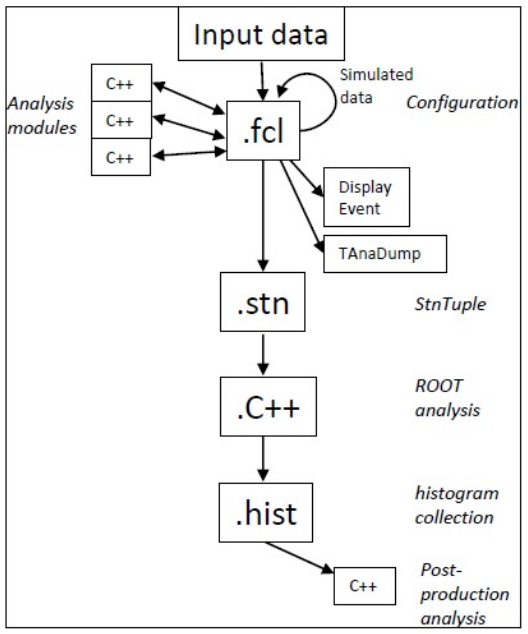
\includegraphics[width =0.4\textwidth]{figures/png/Screenshot_20240809_174458.png}
    \caption[Mu2e simulation and data handling.]{Both the generation and reconstruction 
    of events are performed through art-jobs configured using FHiCLs, which import the 
    necessary C++ modules. Additionally, modules such as the Event Display and TAnaDump 
    are utilized for debugging purposes. The analysis workflow relies heavily on the use 
    of STNTUPLE.
    }
    \label{fig:multistage}
\end{figure}

\section{Multi-stage Simulation}

The Mu2e simulation leverages a method known as multi-stage 
simulation to efficiently generate and simulate events. This 
technique involves generating events, partially simulating them, 
then pausing the process to save the generated data. Subsequent 
stages continue the simulation from the saved state, further 
advancing it before saving again. Multiple stages are often 
required to complete the entire simulation. These stages typically 
conclude when particles reach specific planes or volumes, such as 
the Detector Solenoid (DS) region that contains the target and 
detector, or the tracker volume. This approach is particularly 
valuable when the early stages of the simulation consume the 
majority of CPU time.

The rationale for employing multi-stage simulation includes:

\begin{itemize}
    \item \textbf{Incremental detector definition}: The simulation can 
    incrementally define different parts of the detector in later stages. 
    For example, computationally demanding tasks, such as simulating protons 
    on target, can be handled in an initial stage, allowing the tracker 
    geometry and algorithms to be introduced later. Once the tracker is 
    ready, the simulation can continue into its volume;
    \item \textbf{Efficient design variation studies}: Multi-stage 
    simulation facilitates the exploration of different experimental 
    designs. By concluding simulation stages outside the detector, 
    various detector designs can be tested quickly without the need to repeat earlier stages;
    \item \textbf{Effective error recovery}: This approach acts as a 
    checkpoint mechanism, improving error recovery efficiency. If an 
    error occurs in a later stage, only that stage needs to be re-simulated, 
    using the output from the previous stage. Given that the early stages 
    often require the most CPU time, this can result in significant time savings;
    \item \textbf{Resource and limitation management}: Multi-stage simulation 
    effectively handles constraints such as job duration and output file size. 
    Techniques like compression, event filtering, and concatenation can be used 
    to manage resources efficiently.
\end{itemize}

Multi-stage simulation also supports two critical techniques: mixing and resampling, which are essential for studying backgrounds and processes with low statistics.

For the study of muon beamline vertical misalignments presented in this thesis, the simulation framework is organized into six stages:

\begin{itemize}
    \item \textbf{First stage (s1)}: Simulates the interactions of 
    8 GeV protons with the Production Target (PT), tracing all produced 
    particles that contribute to the beam up to the midpoint of the Transport 
    Solenoid (TS), and saving data for any particles that reach this point;
    \item \textbf{Second stage (s2)}: Uses the output from $s1$ to trace the 
    beam up to the entrance of the Detector Solenoid;
    \item \textbf{Third stage (s3)}: Propagates the surviving particles 
    from $s2$ through the upstream portion of the DS vacuum and records 
    muons that stop in the aluminum Stopping Target (ST);
    \item \textbf{Fourth stage (s4)}: Separates $\mu^+$ and $\mu^-$ 
    stopped in the ST into two distinct outputs for separate analysis;
    \item \textbf{Fifth stage (s5)}: The detector is finally simulated. 
    Muons stopped in the target undergo Michel decays. The resampling 
    technique is applied to increase statistics, using each stopped 
    muon multiple times as a starting point for generating different 
    decays. Particles intersecting the tracker or calorimeter are recorded;
    \item \textbf{Sixth stage (s6)}: Converts the simulated raw data into 
    simple C++ classes or structs, simulating the digitization of detector raw data;
    \item \textbf{Seventh stage (s7)}: The final stage reconstructs particle tracks and generates n-tuples.
\end{itemize}

This multi-stage approach conserves computational resources in the study of vertical 
misalignment effects. For instance, generating datasets with displaced COL3 requires 
only re-running stages 2 onward, which is highly advantageous since $s1$ is the most 
resource-intensive stage.
